\chapter{Conception}

\section*{Introduction}
\qquad Dans ce chapitre, nous nous intéressons à la conception de notre projet. En effet la conception s'avère la pierre angulaire de tout projet appelant à l'ingénierie. En se basant sur la spécification détaillée des besoins, nous allons pouvoir définir tout les éléments faisant partie de la réalisation. Nous préciserons alors les éléments de la conception architecturale ainsi ceux de la conception détaillée.\\

\section{Conception globale}

\qquad Nonobstant la simplicité du besoin de notre application, ce dernier n'est pas aussi évident à réaliser car il fait appel à un certain niveau de complexité architecturale. Généralement notre application est composée de deux majeures parties à savoir : la partie Backend, responsable de tous les traitements possibles, la collecte des données et la réponse aux requêtes des clients, et la partie Frontend qui est la partie déployée chez les utilisateurs qui servira comme une Interface Homme Machine (IHM). La figure \ref{fig3.1} illustre l'architecture de notre système. Nous y revenons en plus de détail par la suite.

\begin{figure}[!h]
	\begin{center}
		\includegraphics[width=0.914\linewidth]{figures/arch}
	\end{center}
	\caption{Architecture globale de l'application}
	\label{fig3.1}
\end{figure} 

La communication entre la partie front et back se fait à base de services Web REST (HTTP et JSON). En fait, la partie Frontend consomme les services web fournis par la partie Backend. (Voir figure \ref{fig3.2})

\begin{figure}[!h]
	\begin{center}
		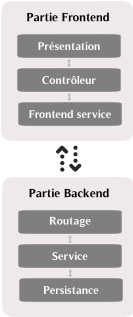
\includegraphics{figures/liaison}
	\end{center}
	\caption{Architecture global de la couche Web}
	\label{fig3.2}
\end{figure}

\subsection{Partie Backend}

\qquad Comme est mentionné précédemment, la partie backend est responsable de la majorité des traitements réalisés par notre application : 
\begin{itemize}
	\item Interrogation de la base de données,
	\item réponse aux requêtes des utilisateurs,
	\item envoie des notifications,
	\item envoie des Emails,
	\item collecte des données publiques,
	\item récupération des informations utiles
\end{itemize}

Elle composée par deux composantes à savoir le serveur HTTP et les applications Batch. Le serveur HTTP fournit des API consommables par la partie frontend par le biais du modèle architecturale REST qui permet la communication entre ces deux parties sur des sockets HTTP usant ainsi les méthodes du protocole HTTP. L'objectifs des applications Batch est d'exécuter des taches bloquantes qui nécessitent beaucoup de temps pour s'exécuter et sont indépendantes de toutes interventions humaines. Typiquement, les Batchs seront utilisés à :
\begin{itemize}
	\item traiter des taches planifiées,
	\item traiter des taches volumineuses (lecture/écriture),
	\item traiter parallèlement des données...\\
\end{itemize}

Notre application utilise les Batch pour les cas d'utilisation suivants :
\begin{itemize}
	\item Recueillir et traiter les données publiques
	\item Interroger les objets Netatmo
	\item Enregistrer les informations utiles dans la base de données
	\item Envoyer les notifications aux utilisateurs
	\item Suivre l'état du serveur Backend
	\item Mettre à jour le fichier log
\end{itemize}

De ce fait, les Batch sont lancés périodiquement ou selon la planification définie par des cron. Les cron sont des programmes qui permettent d'exécuter automatiquement des taches à une date et heure spécifiée à l'avance ou selon un cycle. Seulement le batch d'envoie des notifications est exécuté selon un algorithme paramétré par les niveaux quotidiens de risque.


\subsection{Partie Frontend}

\qquad La partie Frontend autrement désignée par la partie Client sera déployée sur les appareils des utilisateurs et usera les API offertes par la partie Backend pour récupérer les informations nécessaires au rendering des vues (view) de notre application.La partie client est aussi responsable des transitions entre les view. Ainsi à partir des templates préalablement définies la partie frontend crée les Interface Homme/Machine (IHM)  accessibles par l'utilisateur afin de consulter les différentes fonctionnalités offertes par l'application. Outre la présentation et la création des IHM, la partie frontend fournit des services clients tels que l'accès au ressources de l'appareil téléphonique (Géolocalisation, Internet...) (voir figure \ref{fig3.2}).

\section{Conception détaillée}

\qquad Nous présentons dans cette partie la conception de notre application à travers le langage UML. Nous représenterons les diagrammes de modélisation UML.

\subsection{Diagramme de paquetage}
\qquad $\grave{A}$ fin d'assurer la modularité de notre système nous optons pour représenter les relations entre les différentes classes par le diagramme de paquetage. Le diagramme de paquetage assure aussi une meilleur lisibilité du diagramme des classes. Chaque module est alors représenté par un paquet selon le domaine fonctionnel comme le représente la figure \ref{fig3.3}.

\begin{figure}[!h]
	\begin{center}
		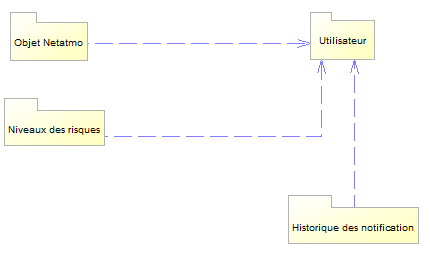
\includegraphics[width=0.64\textheight]{figures/pckg1}
	\end{center}
	\caption{Diagramme de paquetage}
	\label{fig3.3}
\end{figure}
\newpage
\subsection{Diagramme de classes}

\qquad Arrivant à ce stade nous allons décomposer chaque paquet du diagramme de la figure \ref{fig3.3} en diagramme de classes représentant ainsi les relations existante entre les classes de notre projet. Les relation entre les paquets sont représentées par les relations des classes qui les composent. Chaque classe est illustrée par ses attributs et les relations qui la relie aux classes de son paquet parent et des classes des autres paquets.

\subsubsection{Diagramme de classes relatif au paquet : Utilisateur}

\qquad Le diagramme de la figure \ref{fig3.4} représente le modèle des classes du paquet : Utilisateur.

\begin{figure}[!h]
	\begin{center}
		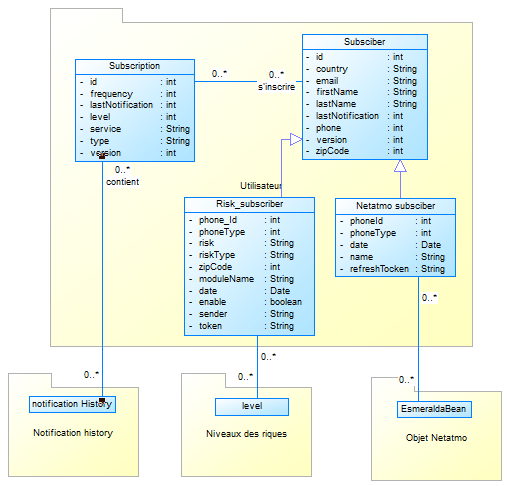
\includegraphics[width=0.64\textheight]{figures/pckg2}
	\end{center}
	\caption{Diagramme de classes relatif au paquet : Utilisateur}
	\label{fig3.4}
\end{figure}
\newpage
\subsubsection{Diagramme de classes relatif au paquet : Niveau des risques}

\qquad Ci-après est représenté la décomposition du paquet Niveau des risques. La figure \ref{fig3.5} illustre les classes membres du paquet : Niveau des risques.

\begin{figure}[!h]
	\begin{center}
		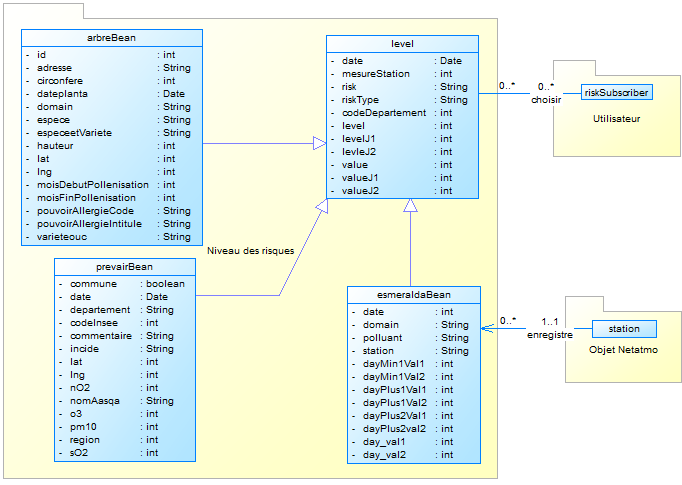
\includegraphics[width=0.64\textheight]{figures/pckg3}
	\end{center}
	\caption{Diagramme de classes relatif au paquet : Niveau des risques}
	\label{fig3.5}
\end{figure}

\newpage
\subsubsection{Diagramme de classes relatif au paquet : Objet Netatmo}

\qquad La figure \ref{fig3.6} illustre le diagramme de classes relatives au paquetage « Objet Netatmo ».

\begin{figure}[!h]
	\begin{center}
		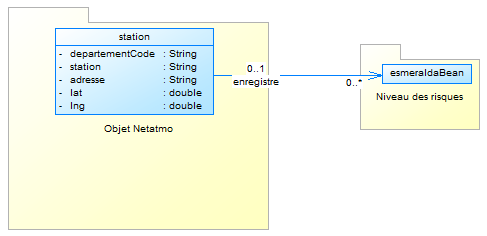
\includegraphics[width=0.64\textheight]{figures/pckg4}
	\end{center}
	\caption{Diagramme de classes relatif au paquet : Objet Netatmo}
	\label{fig3.6}
\end{figure}

\subsubsection{Diagramme de classes relatif au paquet : Historique des notifications}
\qquad Les classes du paquetage « Historique des notifications » sont modélisées dans la figure ci-dessous.

\begin{figure}[!h]
	\begin{center}
		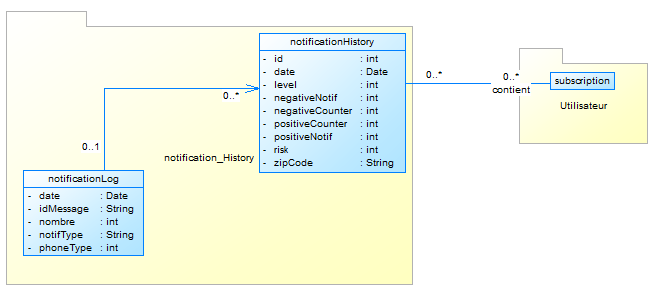
\includegraphics[width=0.64\textheight]{figures/pckg5}
	\end{center}
	\caption{Diagramme de classes relatif au paquet : Historique des notifications}
	\label{fig3.7}
\end{figure}

\subsection{Digrammes de séquence}
\qquad Les diagrammes de séquences permettent de donner une vue dynamique sur l’interaction entre l’acteur et le système. Nous représentons, dans cette section, des enchaînements de quelques scénarios à travers les diagrammes de séquences d’UML.

\subsubsection{Diagramme de séquence "Ajouter astuce"}

\qquad La figure \ref{fig3.8} illustre le diagramme de séquence de la fonctionnalité "Ajouter astuce" dont l'acteur est l'utilisateur et la post-condition est l'ajout d'une astuce. L'ajout d'une astuce se fait à plusieurs étapes. Après avoir accéder à la page d'ajout l'utilisateur interagira avec l'IHM contenant les champs à remplir pour accomplir la tache. Il saisira l'astuce, ses cordonnées (Pseudonyme et mail) et choisira le type de risque. Une fois les champs remplis, il peut confirmer son ajout en appuyant sur le bouton "submit" qui actionnera toute la chaine d'exécution expliquée par le tableau \ref{tab3.1}.


\begin{figure}
	\begin{center}
		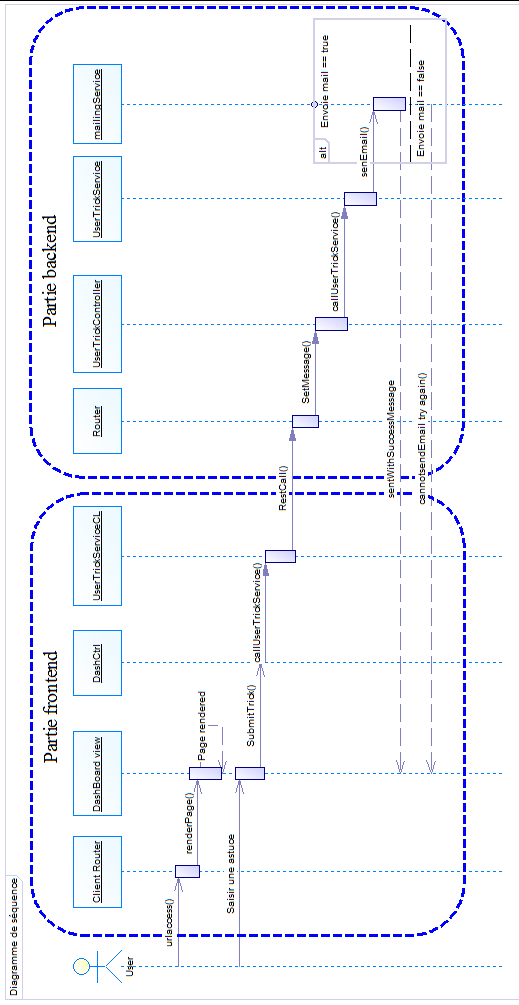
\includegraphics[height=\textheight]{figures/ds1}
	\end{center}
	\caption{Diagramme de séquence "Ajouter astuce"}
	\label{fig3.8}
\end{figure}

\newpage

\begin{table}
	\caption{Description textuelle de la chaine d'exécution de la fonctionnalité : Ajouter astuce}
	\label{tab3.1}
	\begin{center}
		\begin{tabular}{|L{2.2cm}|L{2.8cm}|L{2.8cm}|L{4.7cm}|}
			\hline
			\textbf{Fonction} & \textbf{Emplacement} & \textbf{Action/Fonction appelante} & \textbf{Rôle}\\
			\hline
			submitTrick & DashCtrl & Appui sur le bouton "Submit" & -Vérifie le contrôle sur les champs\\
			& & &-Appelle le UserTrickService\\
			\hline
			addUserTrick & UserTrickService & submitTrick & -Faire l'appel REST au serveur\\
			\hline
			setMessage & userTrickController & addUserTrick & -Appelle le service de constructionde message\\
			\hline
			buildMessage & userTrickService & setMessage & -Construire le message à envoyer pa mail\\
			\hline
			sendEmail & mailingServie & addUsertrick & -Envoyer l'astuce de l'utilisateur vers le mail de SmartData\\
			\hline
			
		\end{tabular}
	\end{center}
\end{table}

\subsubsection{Diagramme de séquence "Télécharger Rapport XLS"}

L'acteur de cette fonctionnalité est l'administrateur. $\grave{A}$ travers ce cas d'utilisation, l'administrateur peut télécharger un rapport sous format .xls de l'état de l'application. Après avoir accéder à l'URI correspondante, une IHM sera affichée qui à travers laquelle peut consulter le rapport sur le Web ou le télécharger en format .xls.

\begin{figure}[!h]
	\begin{center}
		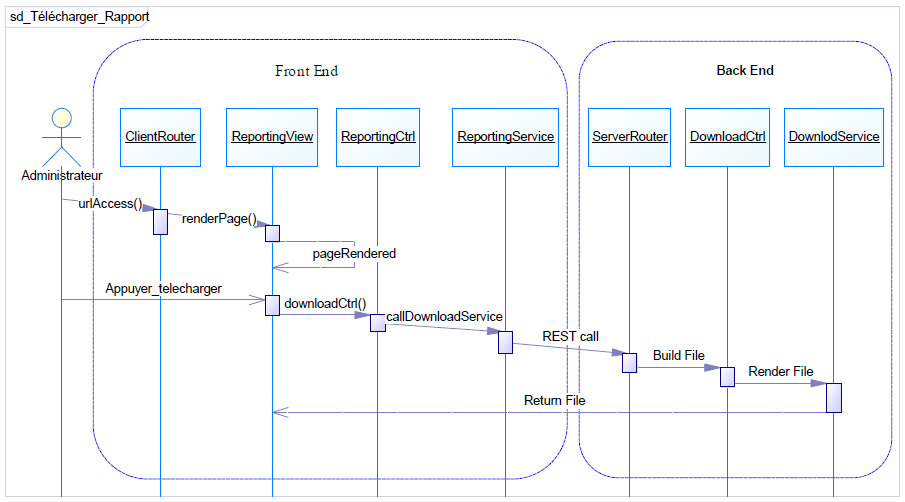
\includegraphics[width=0.64\textheight]{figures/sd2}
	\end{center}
	\caption{Diagramme de séquence "Télécharger Rapport XLS"}
	\label{fig3.9}
\end{figure}

\subsection{Diagramme d'activité}

\qquad Dans cette partie nous présentons, par le modèle du diagramme d'activité, les décisions prises par le système lors de l'exécution de la fonctionnalité "Ajouter Astuce". Nous nous intéressons aux diagrammes comportementaux d’UML. Les
diagrammes d’activités sont utilisés pour modéliser un workflow dans un use case ou entre plusieurs uses cases et pour spécifier une opération ( logique d’une opération ).\\

Le diagramme d’activité est le plus approprié pour modéliser la dynamique d’une tâche ou d’un use case. Nous commençons par montrer le diagramme d’activités relatives aux processus d’authentification et d’inscription puis celles qui sont relatives au processus d’ajout d’un membre.\\

La figure \ref{fig3.10} représente le diagramme d'activité du cas d'utilisation " Ajouter astuce ".

\begin{figure}[!h]
	\begin{center}
		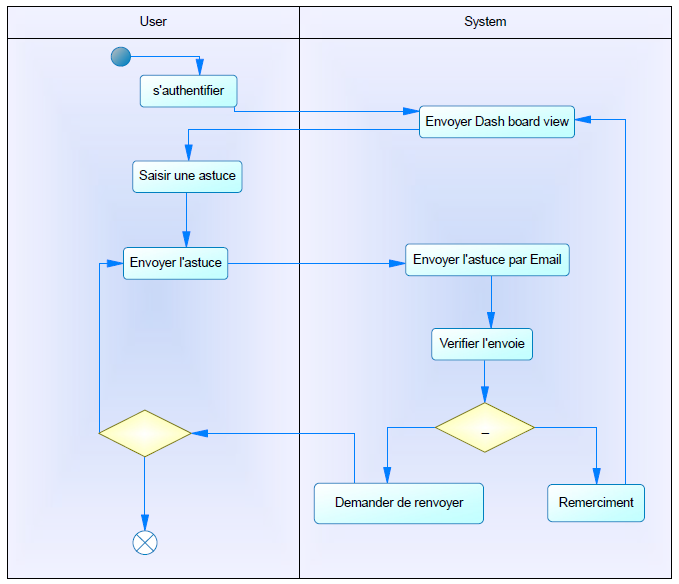
\includegraphics[width=0.64\textheight]{figures/ad1}
	\end{center}
	\caption{Diagramme d'activité du cas d'utilisation " Ajouter astuce "}
	\label{fig3.10}
\end{figure}

\subsection{Diagramme de déploiement} \label{para}

\qquad Un diagramme de déploiement est un diagramme UML qui fournit une représentation graphique de la configuration physique des éléments d'exécution de notre système. En phase de production, l'infrastructure physique nécessaire se compose de quatre parties majeures: 

\begin{itemize}
	\item Le Système de Gestion de Base de Données (SGBD)
	\item Le serveur Web pour la gestion des requêtes, des transactions vers la base de données et le lancement des Batch
	\item L'infrastructure Cloud pour l'exécution des Batch
	\item Les parties clientes : client mobile et client léger qui consomment les API REST de la partie Backend déployée dans le serveur Web.\\
\end{itemize}

La figure \ref{fig3.11} représente les différentes relations entre les parties du système déployés sur l'infrastructure physique ainsi que les protocoles utilisés pour assurer la communication entre les composantes de la configuration.

\begin{figure}[!h]
	\begin{center}
		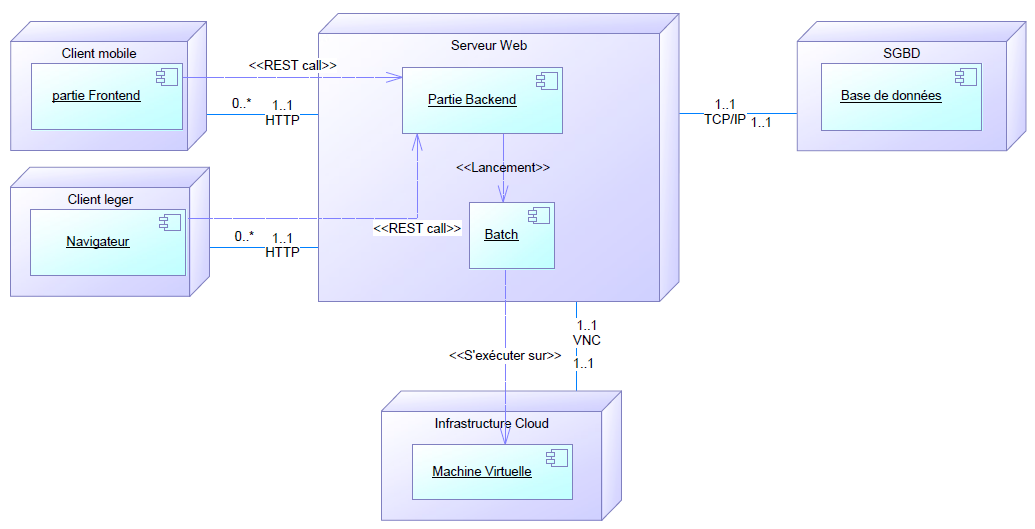
\includegraphics[width=0.63\textheight]{figures/dep}
	\end{center}
	\caption{Diagramme de déploiement}
	\label{fig3.11}
\end{figure}

\section*{Conclusion}

\qquad Nous avons traité dans ce chapitre l’étude conceptuelle de notre système. Nous avons présenté, dans un premier lieu, l’architecture globale de notre application. Puis, nous avons décrit plus en détails les différentes parties du système. Nous entamons à présent la partie relative à la réalisation de notre application.